\documentclass{report}

\usepackage{graphicx} % Required for inserting images
\usepackage{amsmath,amssymb}
\usepackage{tcolorbox}
\tcbuselibrary{theorems, skins}  


\definecolor{maincolor}{HTML}{1E90FF}

\newtcbtheorem{teorema}{Teorema}%
{colback=maincolor!10!white,
 colframe=maincolor!80!black,
 fonttitle=\bfseries,
 coltitle=black,
 boxrule=0.8pt,
 arc=4pt,
 enhanced}{th}

\begin{document}


\section{Introduzione}

In questo corso andremo a vedere le basi della \textbf{Crittrografia moderna}, in primis dobbiamo capire cosa vuol dire "\textit{Crittrografia}. Partiamo dall'etimologia: dal greco \textbf{\textit{kryptós}} (nascosto) - \textbf{\textit{graphía}} (scrittura). In sostanza, la Crittografia è quella disciplina che studia e analizza come inviare e ricevere messaggi \textbf{nascosti}, con il termine "nascosti" si intende che solo ed esclusivamente la sorgente e il destinatario possono leggere il contenuto del messaggio, mentre qualsiasi altra persona non può. 

\begin{figure}[h]
     \centering
    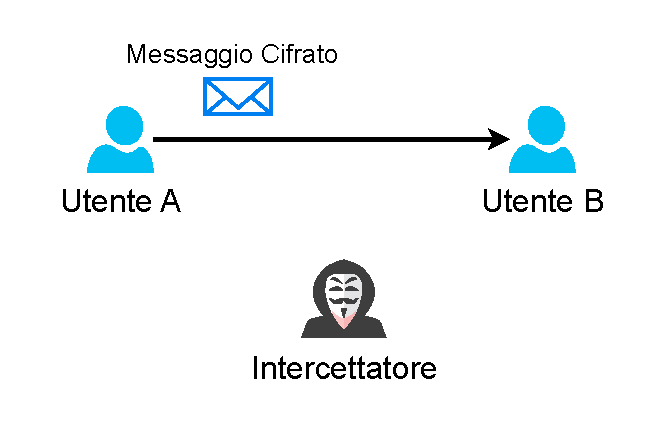
\includegraphics[width=0.6\linewidth]{logos/cripto1.pdf}
\end{figure}

In questa immagine l'utente A manda un messaggio criptato all'utente B, in questa maniera solo A e B potranno leggere il contenuto del messaggio, mentre l'intercettatore anche se riesce ad avere una copia del messaggio non riuscirà a leggerlo l'interno del messaggio (dato che è criptato).

% Le premesse che ha la criptografia sembrano molto semplici ma con calma capiremo che dietro a questa piccolissima premessa si nasconde un mondo tutto da scoprire. 

La Crittografia la usiamo tutti i giorni (anche involontariamente) con i nostri dispositivi elettronici. Un esempio è \textbf{Whatsapp}, che tramite una crittografia \textbf{End-To-End} (che avremo tempo di approfondire) permette di inviare messaggi in maniera sicura, in modo che nessun'altro (nemmeno Whatsapp stesso!) possa leggere il messaggio che hai mandato al tuo amico. Ha anche utilità nell'autenticazione digitale e documenti elettronici, infatti tutti i sistemi come \textbf{SPID} oppure \textbf{CIE} sfruttano la crittografia per funzionare. La crittografia viene utilizzata anche dalle case produttrici di conssole (come \textbf{Sony} per la \textbf{Playstation}) per impedire di crackare le loro console. Di ese,pi ce ne sono a centina e avremo tempo per scoprirli tutti. 

Anche se ho elencato tutti esempi \textbf{digitali}, la crittografia è una disciplina che si basa sulla \textbf{matematica}, infatti tutti i sistemai crittografici struttano prove matematiche (come \textbf{Logaritmo Disceto} e \textbf{Fattorizzazione di numeri composti }) per funzionare. Infatti mi piace definire la crittografia come una branca che sta a metà strada tra matematica e l'informatica, perchè usa nozioni matematiche ma le applica in contesti informatici.

Un altro punto fondamentele da chiarire è che nonostanre parleremo di sistemi moderni come \textbf{AES}, \textbf{RSA}, \textbf{DIffie-Helmann} e \textbf{ECC} che sono stati inventati tra il 1960 e 1990 circa, in realtà la crittografia è molto più vecchia, infatti già dal'\textbf{Impero Romano} (753 A.C. - 476 D.C.) se ne parlava, chiaramente era molto più semplice dei sistemi odierni ma all'ora serviva per mandare messaggi all'esercito. In questo coro di cifrari "antichi" ne vedremo due, forse i più impattanti nella storia: \textbf{Cifrario di Cesare} che possiamo definire come il primo sistema crittografico, e la macchina \textbf{Enigma} che durante la Seconda Guerra Mondiale fu di fondamentele importanza per le truppe dell'Asse, ma gli alleati grazie a \textbf{Alan Turin} riuscirono a rompere la macchina aiutanto gli alleati a vincere la guerra. 

Fatte tutte le premesse del caso iniziamo a parlare di crittografia, e come prima cosa capiamo tutti i termini che si usano in questo ambito.

\subsubsection{Cifratura} La cifratura di un messaggio è il processo che permette di \textbf{alterare} un messaggio che si vuole mandare in maniera che nessun'altro (apparte chi manda il messaggio e il destinatario) possa leggerne il messaggio originario. La cifratura deve avvenire tramite un \textbf{algoritmo di cifratura} e tramite l'ausilio di una (o più) \textbf{chiave}.


\begin{figure}[h]
     \centering
    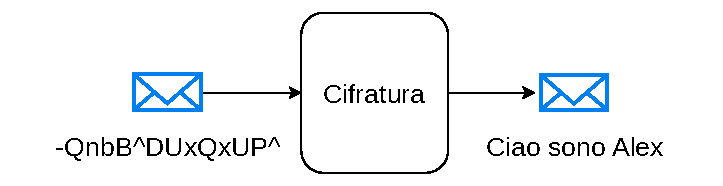
\includegraphics[width=0.8\linewidth]{logos/cripto2.pdf}
\end{figure}


In questo caso il messaggio "\textbf{Ciao sono Alex} tramite una cifratura è diventato \textbf{-QnbB\^{}DUxQxUP\^{}}, se qualcuno riuscisse a intercettare il messaggio cifrato non capirebbe nulla.


\subsubsection{Decifratura} La decifratura è il passaggio \textbf{inverso} della cifratura, nel senso che permette di tornare al messaggio originale avendo il messaggio cifrato. Chiaramente bisogna usare lo \textbf{stesso algoritmo di cifratura} e sopratutto la \textbf{stessa chiave}, che ricordiamo deve conoscerla solo chi manda il messaggio e chi lo deve ricevere.


\begin{figure}[h]
     \centering
    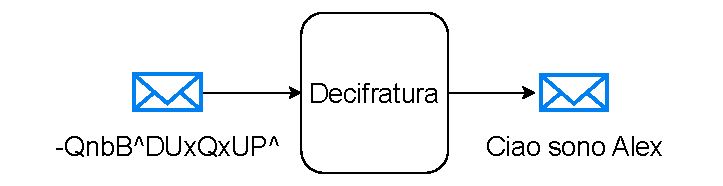
\includegraphics[width=0.8\linewidth]{logos/cripto3.pdf}
\end{figure}


Inizziamo ad usare del nozionismo matematico, il meccanisco di cifratura e decifratura le possiamo paragonare ad una \textbf{funzione} perchè entrambe prendono una variabile in input e restituiscono un valore in output. Quindi possiamo definire la cifratura come 

\begin{equation*}
    c = f(m)
\end{equation*}

Dove $c$ è il messaggio cifrato, $m$ è il messaggio originale e $f$ è la "funzione cifratura". Dato questo allora la "funzione decifratura" sarà definita come

\begin{equation*}
    m = f^{-1}(c)
\end{equation*}

Questo si può dedurre dalla seguente equazione

\begin{equation*}
    m = f^{-1}(f(m)) 
\end{equation*}

Tranquilli per ora abbiamo finito con il nozionismo matematico. Per ora.


\subsubsection{Chiave} una chiave è una qualsiasi \textbf{stringa} o anche più sempliceemnte un \textbf{numero}, ma la caratteristica principale è che una chiave deve \textbf{rimanere privata}, perchè la chiave permette di criptate e ddecriptare i messaggi, quindi se qualcuno riesce a rintracciare la vostra chiave privata vi potrà leggere tutti i messaggi che mandate e che ricevete. L'idea della chiave in crittografia è uguale alla \textbf{password}, infatti alla stessa maniera se qualcuno vi ruba la password vi può entrare nell'account. In realtà la chiave può anche essere un qualcosa si più complicato: come un \textbf{punto nel piano cartesiano} (usato nella \textit{Elliptic Curve Cryptografy}). 

Quindi per evitare confunsione correggiamo la definizione di prima dicendo che una chiave è un qualsiasi \textbf{dato}, oppure un \textbf{insieme di dati},  che deve rimanere \textbf{segreto}.

In realtà vedremo verso metà corso che esiste anche una così detta \textbf{chiave pubblica}, ovverò una chiave come la abbiamo definita fino ad ora ma \textbf{chiunque la può sapere}. Se vi sembra strano e contro intuitivo quando lo vedremo sarà tutto chiaro.

\subsubsection{Rotto} un sistema crittografico si definisce \textbf{Rotto} qualora si riesca a decifrare un messaggio criptato senza la chiave. Un sistema rotto chiaramente non si può usare perchè chiunque riuscirebbe a decriptare il messaggio. Un esempio di sitema rotto è il \textbf{DES} (che vedremo nel capito Cifrari a Blocchi). Il DES è stato inventato nel 1976 e all'inizio era molto usato, ma il problema è che usava una chiave a lunghezza fissa: 54 bit. Ad oggi purtroppo una chiave a 54 bit è soggetta ad attacchi \textbf{brute-force} \footnote{Attacchi in cui si provano tutte le possibili combinazioni di una chiave, chiaramente richiede molto tempo ma per chiavi molto piccole (come DES) può funzionare} e per questo oggi non si può più usare il DES per cifrare ed è stato stituito dall' \textbf{AES}.





\newpage

\subsection{Principio di Kerckhoffs}

Ora che abbiamo iniziato a masticare i primi termini della Crittografia possiamo capire il prinicpio fondante della crittografia: \textbf{Il Principio di Kerckhoffs} (Occhio a non leggere kirchhoff che riguarda elettronica).

\begin{teorema}{Principio di Kerckhoffs}{}
la sicurezza di un sistema crittografico deve dipendere unicamente dalla chiave segreta, e non dalla segretezza dell'algoritmo stesso
\end{teorema}

Sostanzialmente Kerckhoffs dice che non deve essere segreto \textbf{l'algoritmo di cifratura} ma la forza di un sistema crittografico è data dalla difficilità di rompere il sistema stesso, e non dalla segretezza dell'algoritmo.

Per questo motivo noi oggi sappiamo perfettamente come che algoritmi usano i vari siti/app perchè non è un rischio sapere come viene criptato il messaggio, ma la sicurezza sta nella segretezza della chiave che quella chiaramente deve rimanere segreta.

Per esempio per Kerckhoffs, se te e un tuo amico volete creare un sistema per potervi scambiare messaggi segreti, non potete usare un sistema debole ma mantenendolo segreto a tutti gli altri, anche perchè se qualcuno riuscisse a scoprire l'algoritmo vi leggerebbe tutti i messaggi.




\subsection{Il problema dello scambio della Chiave}

Prima di cominciare a parlare della classificazione dei sistemi crittografici, serve che parliamo del problema dello scambio della chiave. Ripetendo quanto visto fino ad ora, la crittografia studia come due utenti possano scambiarsi dei messaggi in maniera che nessun altro ne possa leggere il contenuto e abbiamo capito che il messaggio viene crittato, e poi decriptato, tramite un algoritmo. Abbiamo anche capito che un algoritmo ha bisogno di una chiave per poter cifrare i messaggi, e la chiave la deve avere solo chi manda il messaggio e chi lo deve ricevere e nessun altro (altrimenti anche altri utenti potrebbero decrittare i messaggi), però non abbiamo ancora pensato come i due utenti possano scambiarsi una chiave comune, o comunque mettersi d'accordo su una chiave da usare per il sistema.

\begin{figure}[h]
    \centering
    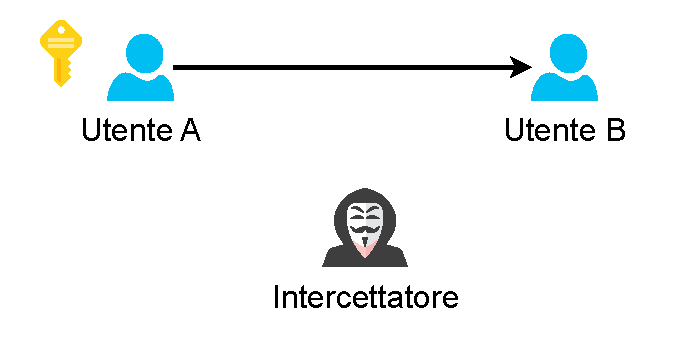
\includegraphics[width=0.6\linewidth]{logos/critpo5pdf.pdf}
\end{figure}

In questa immagine l'utente A ha generato una chiave da usare per crittare i messaggi ma deve trovare un modo per inviarla a B (così che lui possa decrittare i messaggi di A) senza che l'intercettatore riesca ad avere la chiave. Questo problema è stato risolto tramite i sistemi \textbf{Asimmetrici}, come sia possibile lo vedremo quando li studieremo nel dettaglio, per ora vi basta sapere che questo problema dello scambio è risolto da questi tipi di sistemi.




\subsection{Le prime Classificazioni}

I sistemi crittografici si dividono in molte sottocategorie, ognuno con le sue caratteristiche. Per comprenderle meglio vediamo subito una mappa riassuntiva su tutte le categorie, e poi le commentiamo una ad una, perciò ecco a voi la mappa

\begin{figure}[h]
    \centering
    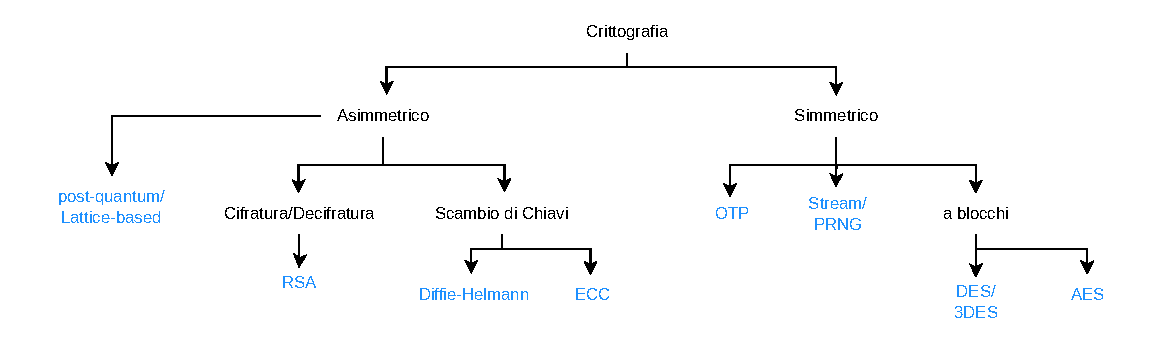
\includegraphics[width=\linewidth]{logos/cripto4.pdf}
\end{figure}





La prima grande distinzione nella crittografia moderna è la differenza tra sistema \textbf{Simmetrico} e \textbf{Asimmetrico}. Un sistema simmetrico utilizza \textbf{una sola chiave} che deve rimanere sempre privata, mentre i sistemi asimmetrici hanno \textbf{2 chiavi: una privata e una pubblica}. I due sistemi sono uno complementare all'altro e ora vedremo le principali pro e contro di entrambi.

Sistemi Simmetrici:

\begin{itemize}
    \item Sono veloci computazionalmente, nel senso che i computer sono veloci da compiere gli algoritmi di cifratura e decifratura, infatti questi algoritmi usano delle combinazioni di operazioni booleane (come lo \textbf{XOR}) e operazioni su matrici, conti che i computer sanno fare in maniera eccellente. In certi casi c'è la possibilità di parallelizzare dei passaggi per velocizzare ulteriormente
    \item Non risolvono il problema dello scambio della chiave 
\end{itemize}

Sistemi Asimmetrici:

\begin{itemize}
    \item Risolvono il problema dello scambio della chiave, nel senso che questi sistemi non hanno bisogno che i due utenti si siano scambiati la chiave.
    \item Sono più lenti computazionalmente, perchè devono fare operazioni con numeri enormi (parliamo di numeri a 600 cifre!)
\end{itemize}


Queste intanto sono le prime differenze tra asimmetrici e simmetrici, e vediamo che sono complementari, infatti difficilmente nei progetti si usa solamente uno o l'altro, perchè è meglio usare entrambi. Per esempio, il protocollo \textbf{HTTPS}, che serve per inviare le pagine web in maniera crittata, crea una chiave per un sistema \textbf{simmetrico} ma la chiave viene crittata tramite un sistema \textbf{asimmetrico}, in questa maniera i due utenti avranno la chiave in \textbf{maniera sicura} (perchè è stata inviata tramite asimmetrico) ma nella comunicazione viene usata un sistema simmetrico perchè è più \textbf{veloce}.

\subsubsection{Sistemi Simmetrici - OTP}

Tra le due categorie, i sistemi simmetrici sono i primi che vedremo perchè sono tendenzialmente più semplici. Come si vede dal grafico, i simmetrici si dividono in altre 3 categorie: \textbf{OTP}, \textbf{Stream} e \textbf{a Blocchi}. Il primo che vedremo è \textbf{OTP} (\textit{One Time Pad}) e sarà l'unico sistema che è definito \textbf{perfettamente Sicuro}, ovvero che partendo dal messaggio cifrato (senza la chiave) è impossibile ritornare al messaggio originario. Mentre tutti gli altri sistemi che vedremo con attacchi \textbf{brute-force} si può risalire al messaggio originale senza la chiave di cifratura. Chiaramente gli attacchi sono infattibili perchè richiederebbero anni per decifrare, ma nell'ipotesi di avere un computer infinitivamente potente, il cifrario OTP sarebbe l'unico \textbf{impossibile} da tornare al messaggio originario. 

Dopo questa definizione potreste pensare che potremmo usare sempre e solo l'\textbf{OTP} ma purtroppo ha un pecca che lo rende inutilizzabile: che bisogna cambiare sempre chiave dopo ogni cifratura, perchè con l' OTP se due messaggi sono stati cifrati con la stessa chiave, tramite delle \textbf{criptoanalisi} si può risalire alla chiave e ai messaggi originali. E se qualcuno pensanse di generare sempre nuovi chiavi diventerebbe eccessivamente pesante e insostenibile per una comunicazione.


\subsubsection{Sistemi Simmetrici - PRNG / Stream}

La categoria successiva riguarda è quella degli \textbf{Stream}, che però vedremo pochissimo perchè non sono utilizzati. Semplicemente gli Stream funzionano generando un \textbf{flusso} (per questo motivo prende il nome di \textit{Stream}) di \textbf{Numeri Casuali}, e questi numeri casuali vengono usati per cifrare tramite \textbf{OTP} i messaggi. Il problema che la generazione di numeri casuali per i computer è \textbf{impossibile} infatti i computer sono sistermi \textbf{deterministici}. Infatti per generare dei numeri per questo sistema si usano algoritmi detti \textbf{PRNG} (\textit{Preudo Randomic Number Generator}) che provano a generare numeri che sembrano casuali ma che comunque hanno delle correlazioni tra di loro e questo con determinati attacchi si può trovare i numeri successivi allo stream anche senza chiave. Per questo motivo questa tipologia di cifrari oggi non sono per nulla usati.

\newpage
\subsubsection{Sistemi Simmetrici - A Blocchi}

Finalmente arriviamo ai veri sistemi simmetrici: Quelli a blocchi. Questi cifrari sono quelli che vengono usati oggigiorno per la loro sicurezza e \textbf{velocità}. Ad ogni modo i cifrari a blocchi si basano rompendo il messaggio in blocchi a n bit. Supponiamo di voler criptare il messaggio a 120 bit e noi abbiamo un cifrario a blocchi che prende blocchi da 50 bit. Allora vuol dire che il nostro messaggio \textbf{sarà diviso in 3 blocchi: } primo da 50 bit, secodno da 50 bit e l'ultimo da 20 bit, poi l'ultimo se non è grande quanto il blocco del cifrario vengono aggiunti degli zeri (o un qualsiasi \textbf{padding}) in modo che raggiunga la lunghezza di 50 bit.

\begin{figure}[h]
    \centering
    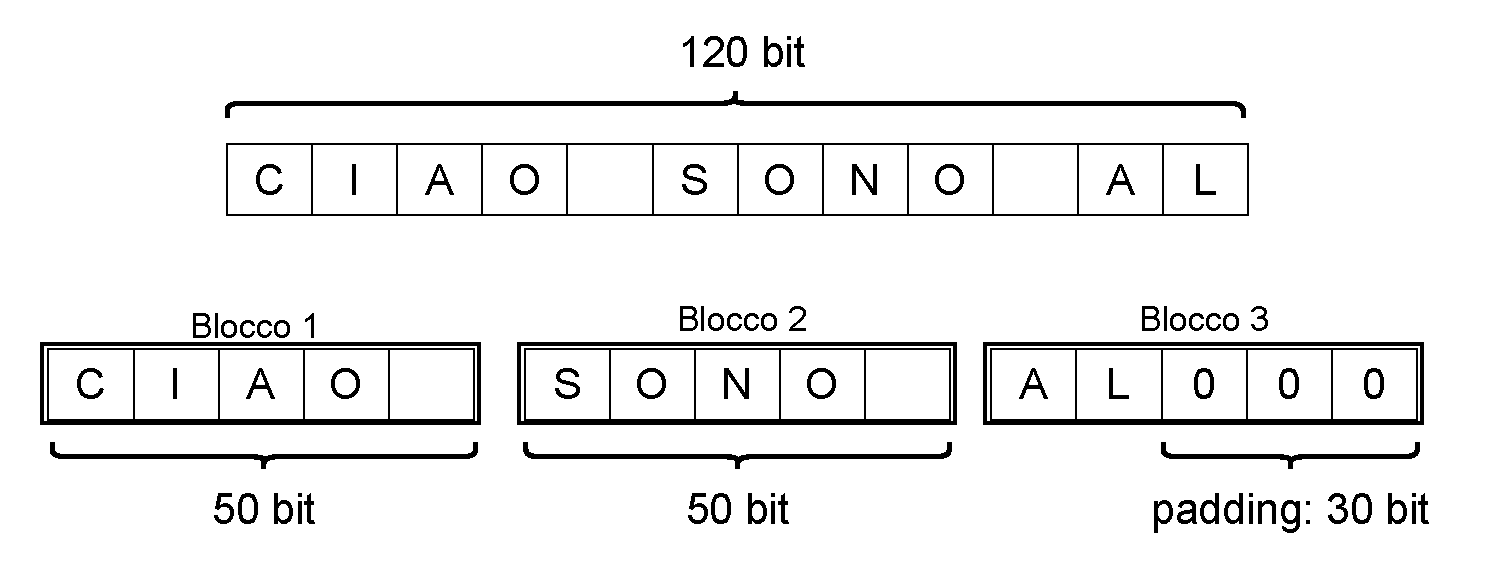
\includegraphics[width=\linewidth]{logos/cripto6.pdf}
\end{figure}



Questo meccanismo di creare dei blocchi serve perchè poi i blocchi vengono trasformati in \textbf{matrici} ed è per questo che serve che abbaiano una grandezza definita, perchè gli altoritmi in sè sfruttano operazioni su matrici per criptare il messaggio, e alla stessa maniera il messaggio cifrato sarà anch'esso una matrice grande uguale che viene riportato a messaggio. è importante capire che visto che l'algoritmo prende un blocco alla volta e lo cripta e chiaramente allo stesso blocco equivale lo stesso blocco cifrato, quindi vuole dire che se due blocchi all'interno del messaggio sono uguali avranno lo stesso blocco cifrato. 


\begin{figure}[h]
    \centering
    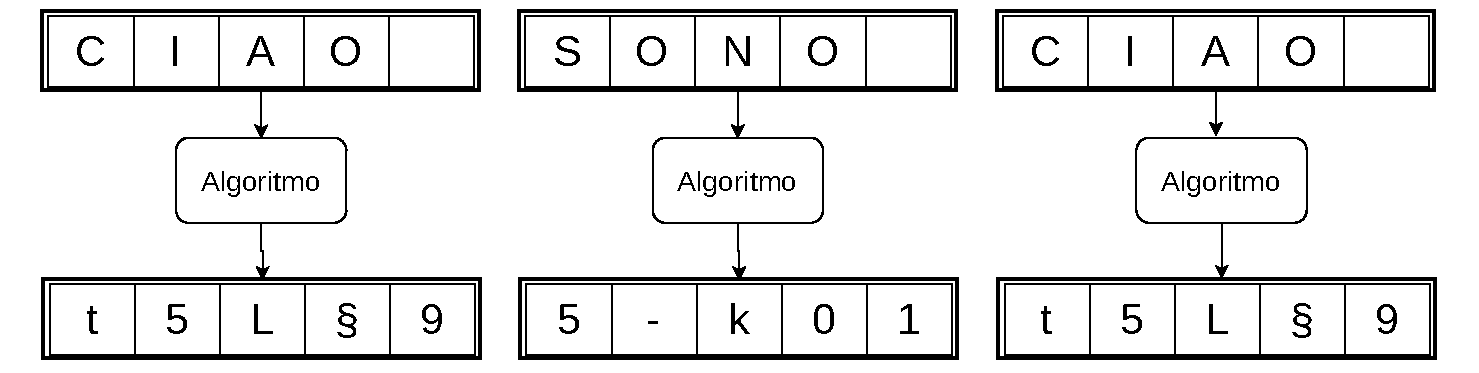
\includegraphics[width=\linewidth]{logos/cripto7.pdf}
\end{figure}

E poi i blocchi cifrati vengono riuniti per formare il messaggio cifrato. Per evitare che due blocchi uguali forniscano lo stesso output (perchè potrebbe aiutare per capire il messaggio originale) si sono inventati i \textbf{Modi di Funzionamento dei cifrari a blocchi}, che vedremo con calma cosa vogliono dire.

La forza di questi cifrari è che usano soltanto operazioni \textbf{booleane} (\textbf{and},\textbf{or}, \textbf{xor} e \textbf{not}) e operazioni \textbf{tra matrici}, il chè le rende molto veloci visto che queste operazioni  sotto ottimizzate nei computer odierni

I principali algoritmi a blocchi sono \textbf{DES} (\textit{Data Encryption Standard}) e \textbf{AES} (\textit{Advanced Encryption Standard}). Il nacque nel 1976 e per i successivi ventanni fu lo standard per i cifrari a blocchi, nel 1999 però dei ricercatori riuscino a \textbf{rompere} il cifrario rendendolo insicuro per via della poca lunghezza della chiave, che permetteva un attacco brute-force. Al suo posto arrivo \textbf{AES} nel 1998 che ad oggi è ancora un sistema sicuro. In più riuscirono a "sistemare" il DES inventando il \textbf{3DES} (\textit{Triple DES}) che non è altro che un messaggio cifrato 3 volte con il DES, e ad oggi questo scamotaggio permette al DES di essere usato ancora (ovviamente oggi si usa solo i 3DES e non più il DES singolo).


\end{document}